\subsubsection{Addition Operator}

This test reveals the native speed of a specific language by doing the most simple of things, addition. The test takes a certain amount of elements and calculates the sum of them. See Figure \ref{fig:native_addition} for results.

\begin{figure}[h]
	\centering
	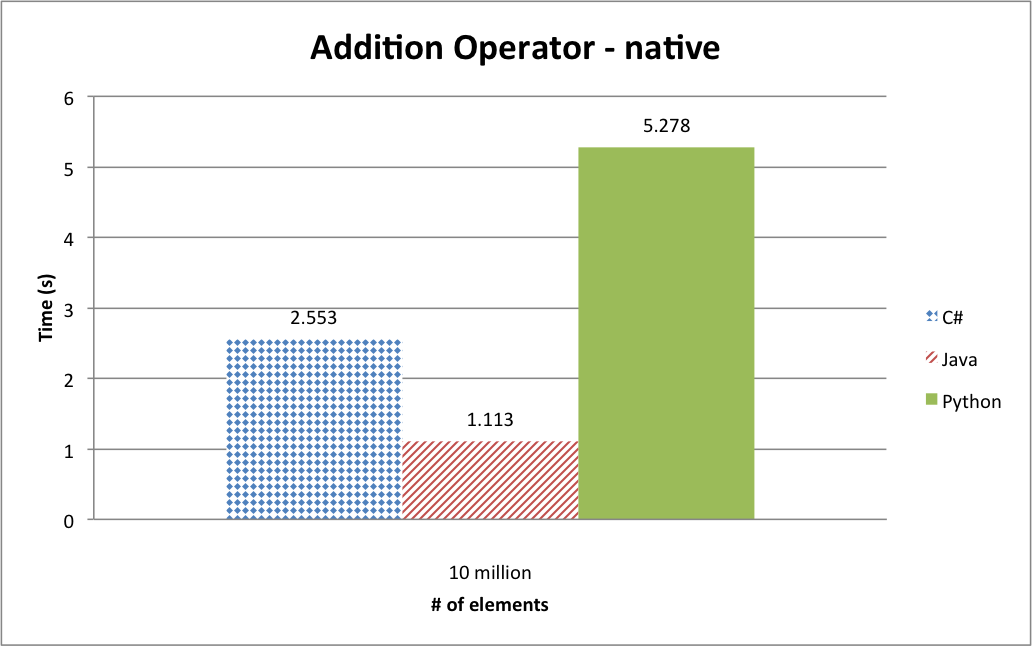
\includegraphics[width=1.0\linewidth]{chapters/new_media/AdditionOperatorNative.png}
	\caption{This tests a language ability to sum 10 million elements. The results show that Java running in its native environment was the fastest of the three languages with 1.113 seconds. Python was the slowest of the three with a runtime of 5.278 seconds, even when using its native library functions to sum the elements, see \ref{appendix:code_addition}.}
	\label{fig:native_addition}
\end{figure}
